\chapter{Intersectional insights}

It is evident that we need another theory to explain what we are seeing, of plain sight. We still emphasize the need toward which the new theory can go, and the backward compatibility that is needed of such. Thus, this section will going through ground zero. We would not try to create the theory right away, but reformulate what has been seen first; this includes even the classical generalization and empirical optimization process, under different interpretations. Some of those results might not fit the formalism, or rather rigorously proven system, yet will ultimately form a logical framework on which developments can be made, and perhaps later on theorems to reaffirm the thesis. But the general idea is simple: \textit{learning is not just approximation}, but an entirely paradoxically simple yet complex construct. 

Specifically, in the first few sections, the fragmented insight would have to be considered, namely of the following dilemma: 

\begin{enumerate}
    \item We need a more general consideration between the environment and the agent, i.e. between the structures $c$ required to extrapolate, and the modulus in which $h$ explicitly exhibits such 'replica' trace. 
    \item Information destruction between encoding and modelling assumptions must be addressed, to accommodate the argument about cross-system information divergence or convergence, and so on. This includes also distribution shift and different kind of mechanistic fits. 
\end{enumerate}

Those are fragmented realization of the development of learning theory, especially with more experiments conducted ever since the developmental framework (\cite{Vapnik1999-VAPTNO,10.1145/1968.1972} are now at least two decades old). The new theory must then, seed such understanding and factors into places, thus also hints at certain type of structural analysis that can conduct such approach. Prerequisition on such structural conditions, the firstly-analysed aspects of consideration includes:

\begin{enumerate}
    \item To capture uncertainty naturally of mathematical modelling descriptions. That is, the mechanistic to probabilistic transition is inherently decomposable, and such transition from white-box and black-box can be captured by different configurations of space. 
\end{enumerate}

Before moving on, we emphasize the importance of realizing the gap between theory and practice. This is inherently serious, and if not for context, should have been included at the very top of the paper. Nevertheless, it should be emphasized here. Critically, this is not rare, and is inherently a complex matter, as seen in many tangent fields and analysis, of \cite{semmelrock2023reproducibilitymachinelearningdrivenresearch,KAPOOR2023100804} on reproducibility and experimental leakage, \cite{Kliemann2016,Tamassia1997ACS} on the engineering reality of algorithms (or geometric algorithms), \cite{bgpt2024} goal on determining the gap between theory and practices, \cite{Revol_2014,COLLANGE201583,Diethelm2012} on numerical reproducibility limits and overall empirical safety, \cite{Kaskenpalo_2012} on theoretical-practice bridge. On the specific side of the theory, \cite{holk2025statisticalguaranteesdenoisingreflected} analysed such statistical guarantee between the theoretical and empirical mistmatch, of which found certain problems regarding such gap, for example, the convergence rate in difussing controlled setting (statistically and system-addess wise, stable); so is \cite{adcock2021gaptheorypracticefunction} on the gap between theory and practice in function approximation with deep neural networks; and so is also \cite{saxena2025aimismatchesidentifyingpotential}, but on the examination of AI mismatches, which usually is concerned of the \textit{implementation details}. Interestingly, \cite{behrouz2025nested} paper on nested learning exploits the line of argument on the mismatch, but however, is troublesome in their formulation and the disparity between theory and practice is not actually addressed, but simply metrics in which the new model is compared to the previous models. That said, it is clear, that any attempt to build theory will inherently attain certain amount of presumptions, implementation decisions, language, memory hierarchy, compiler behaviours, cache, practical limitation on hardware and platorm, and the environment tested in which the model is captured of its results. Even when the theory can be correct, such can also be a factor, coupled with the side of uncertain given when learning process or any stochastic, long-runtime system run for a long time. Such also suggests us to consider the agenda of the \textbf{ergodic theory} in touch. 

\section{Interpreting the learning theory}

Most of the paper will argue about different features of statistical learning theory (\cite{Sterkenburg_2024,Vapnik1999-VAPTNO,STL_Hajek_Maxim_2021}). It is then imperative to discuss the background setting of such. On one hand, when talking of the details on statistical learning theory and the understanding of the encoded language to describe the learning action, typically we are given the observations, or dataset of the form $\mathcal{S}=(\mathcal{X},\mathcal{Y})\subset \mathbb{R}^{n}\times \mathbb{R}^{m}$, of all 2-tuple pairs, assumed to be sampled or observed and governed by a distribution $\mathcal{D}$. On the other hand, there is also the push toward a more general and sophisticated view, in which might as well reveal deeper or richer structures on the theoretical framework to realize. Note that this contains reformulation, or unification, reinterpretation or patchworks of existing structures too, and not simply claimed to be entirely new. 

\subsection{Domain and process}

In dataset, between the \textit{actual concept} and the observable spaces, lies the empirical and generalization setting. While it is not often mentioned in literatures, the switch to direct observable evaluation of statistical learning, induces certain limitations. 

Let us assume the following preliminary in discussion. We have two polars, on the mechanistic absolute, or \textit{white box} knowledge, with full expressions on the underlying mechanics of a certain system concept. Explicitly, this can be written as $y=F(x;\theta)$ under standard morphism, for any kind of description $\theta$. Extension of such notion can also include what we call as the mechanism, or $F(x;\theta,\Gamma)$ of which complies both the parameters, and the formulations. The other polar is the \textit{probabilistic domain}, of which then, we have the inference $\sim$ operator instead. Thus, we denote $y\sim \mathbb{P}(Y\mid X)$ in typical notation, in which the dependency is now $Y$ on the basis of $X$. One can also do the reverse, as to generate the inverse conditions, but this is more probably general, if one switch to joint distribution $(X,Y)$ under statistical schemes. Abstractly speaking, the dual structure contains what we call temporary, as the \textbf{system action} $A_{S}$. The notation then becomes 
\begin{equation}
    yA_{S}x \to f(x;\theta,\Gamma), \quad yA_{S}\to \mathcal{S}[\mathbb{P}(X,Y)]
\end{equation}
For $\mathcal{S}$ here temporarily denotes the \textit{sampling operations}, of observing randomly on the basis of said probability without any knowledge but the presumed parameters. If such process is with control parameter, from the optimization perspective, we have the notation as different to be $\mathcal{S}[\mathbb{P}(X,Y);\theta_{P},\Gamma_{P}]$, where now $\Gamma_{P}$ is the probabilistic process, i.e. distributions or other random structure, for example as stochastic processes as a finite-dimensional distributions plus regularity structure, for random variables $\theta_{P}$. In general, we call it the \textbf{black-box} domain. 

If we are to recover $\theta$ from $\theta_{P}$, or at least on the similarity metric, typically or ML encoded by $\ell(\theta,\theta_{P})$, where $\ell(\theta,\theta_{P})\approx 0$, then we say that the system experiences a \textit{white transition}. Note that we do not take into account of $\Gamma$ and $\Gamma_{P}$, since they are inherently different in this white transition, but mechanistically recoverable; thus, \textit{total white transition} means $\Gamma \approx \Gamma_{P}$ of the mechanistic patterns. If the reverse happens, where mechanistic system turn to probabilistic $(X,Y)$ distribution on $\theta_{P}$ and structure $\Gamma\to\Gamma_{P}$. 

Probability inherently, similar to mechanistic $\Gamma$, enforces causal or rather transformational relation (simply the dual $x\to y$ is transformational within $f$). There, the probability can be interpreted, for either $\Gamma$ explicitly states that they are conditional, for $X$ to be deterministic and explicitly stated, or joint distribution and so on. However, the interference in such recovering mode comes from observational space inconsistency. This is usually expressed of \textit{noise}, where if we admit $(x,y)$ of the mechanistic system, then for $x+\epsilon_{x}$ and $y+\epsilon_{y}$ we have instead a \textit{noisy mechanistic system}. We would note that this is a larger class than pure mechanistic system, basically $x\to [\epsilon, f(x;\theta,\Gamma)]$ instead. Thus, for intrinsic noise of measurements or statistical information, probabilistic transition in recovery of mechanistic systems admits the recovery of the noisy system instead. Depends on the severity of $\epsilon$, such system can be irrecoverable. If such approximation is impossible within certain margin, then probabilistic approximation remains in probable the only manageable system of approximation, rather than a quasi mechanistic recovery mode (we will prove this in a later theorem). 

If we to accept such view, then it means that in certain failure modes, you \textit{cannot move a mechanistic (deterministic) system into probabilistic then back}, given enough disturbance and noise. This quantifies to the \textit{information loss} system-wide, where we can create a prototypical functional, denoted $\mathcal{R}:F\to P$, where
\begin{equation}
    \mathcal{R}[F](A) = \int_{\Theta} \bf{1}_{\{F(x;\theta,\Gamma)\in A\}}\mu (d\theta)
\end{equation}
for such transition, of the probabilistic measure space $(\Omega, \mathcal{F},\mathbb{P})$, for $\mu\in \mathcal{F}$ and $A\in(\mathcal{X},\mathcal{Y})$ of the observational space. The implication here is that, under no information (information-agnostic), every noisy concept must meet certain limit on the basis and resultant structure itself. There exists, presently, no sufficient guarantee to return $P$ to $F$, except the same operation in reversal, is forced on ideal setting, for infinite-range coverage, and approximately dense observational space. The limit is, inherently, enforced by arbitrary $\epsilon$. 

It is to note that we do not claim that mechanistic systems are ontologically privileged; we claim that the mapping from mechanisms to observations is not generally invertible under disturbance.

\subsection{The learner's encoded setting}

Previously, we say that we have the dataset, or rather called as \textbf{observations} of a given system $c$, $\mathcal{S}_{m}$ of size $m$, such that $(x,\cdot)\sim \mathcal{D}$ of a distribution, optionally of also $y$ to be sampled from such distribution. The dataset itself contains pairs, as
\begin{equation*}
    \mathcal{S} = \{ (x_1,y_1), (x_2, y_2),\dots(x_n,y_n) \} \subset \mathcal{X}\times \mathcal{Y}
\end{equation*}
where the dataset is assumed to be i.i.d. sampled according to $\mathcal{D}$, which is unknown by the priori. Hence, we have the first set of assumption. This assumption, based on earlier insight, situated our finding or analysis into the range of black-box and probabilistic models. 
\begin{assumption}
The observational space is governed by a particular sampling distribution $\mathcal{D}$, for fixed $y$-response according to the concept $c\in \mathcal{C}$. The sampling process is further assumed to hold no further structure, hence is \textit{identically and independently distributed} (i.i.d.). 
\end{assumption}

The learning problem is then formulated as followed. Given the machine learning model expressed a hypothesis $h$ of the hypothesis class $\mathcal{H}$, the learning theory aims for creating a procedure to learn either elements of the concept class $\mathcal{C}$ of all concepts $c: \mathcal{X}\to \mathcal{X}$, or the function class $\mathcal{F}$ of all functions $f: \mathcal{X}\to \mathcal{Y}$, which is usually set to $\{0,1\}$ or $[0,1]$. This distinction is trivial, hence, if it is clear, we will talk about the concept class $\mathcal{C}$ only as representative form. The learner $\mathcal{L}(h)$ consider the set of possible hypothesis $\mathcal{H}$, in which might not coincide with $\mathcal{C}$. It receives a partial image of sample $S=(x_{1},\dots,x_{2},\dots,x_n)$ drawn i.i.d. according to $\mathcal{D}$ as well as the label $(c(x_1),\dots,c(x_n))$. This constitutes the dataset $\mathcal{S}$, which are based on specific concept $c\in \mathcal{C}$ for the hypothesis to learn. The task is then to use (or \textit{extract}) meaningful information to select a hypothesis $h_{S}\in \mathcal{H}$ that accurately mimic $c$, with marginal error $\Theta$. The notation $h_{S}$ stands for all hypothesis that can be inferred from the range of the dataset (the first argument, $\mathcal{X}$). 

The marginal error $\Theta$ is considered of two parameters, the empirical error $\hat{R}(h)$ and the generalization error $R(h)$. We give the following definition of them. 

\begin{definition}[Empirical risk]
    Given a hypothesis $h\in \mathcal{H}$, a target concept $c\in \mathcal{C}$, and a sample $S=(x_{1},\dots,x_{m})$. For some particular $\epsilon>0$, the \textbf{empirical error} or \textit{empirical risk} of $h$ is defined by\begin{equation}
        \hat{R}_{S}(h) = \underset{x\in S\sim\mathcal{D}}{\mathbb{P}} [\ell\{h(x),c(x)\}\geq \epsilon] =\frac{1}{m} \sum_{i=1}^{m} \ell\{h(x_i),c(x_i)\}
    \end{equation}
\end{definition}

The generalization risk is then defined as the extension of the empirical risk, of which instead of being evaluated on the set $\mathcal{S}$, it is evaluated on arbitrary infinite density sample space. The notation for the risk calculation can also be $R_{\mathcal{S}}$ instead, of which the need is to classify the set of which it is evaluated from. 

\begin{definition}[Generalization risk]
    Given a hypothesis $h\in\mathcal{H}$, a target concept $c\in\mathcal{C}$, and an underlying distribution $\mathcal{D}$ on $\mathcal{X}$. For some particular $\epsilon>0$, the generalization error or \textit{risk} of $h$ is defined by
    \begin{equation}
        \begin{split}
          R(h) 
          &= \underset{x\sim\mathcal{D}}{\mathbb{P}} [\ell\{h(x),c(x)\}\geq \epsilon]\\
          &= \underset{x\sim\mathcal{D}}{\mathbb{E}}[\ell\{h(x),c(x)\}]\\ 
          &= \int_{x\in \mathcal{D}} \ell\{h(x),c(x)\} \: dP(x)
        \end{split}
    \end{equation}
\end{definition}

In essence, the empirical risk measure the hypothesis to observation error, and the generalization risk captures the difference of the hypothesis to the actual concept. Notice that by doing this, we have implicitly assumed that the observations and the concept is not the same thing, under the majority of scenarios. For the observations to be \textit{approximately equal} or sufficiently captures the concept, there then would have to be various criteria to fulfil. This can be illustrated as Illustration~\ref{fig:statlearnclassical}. 
\begin{figure*}
  \centering
  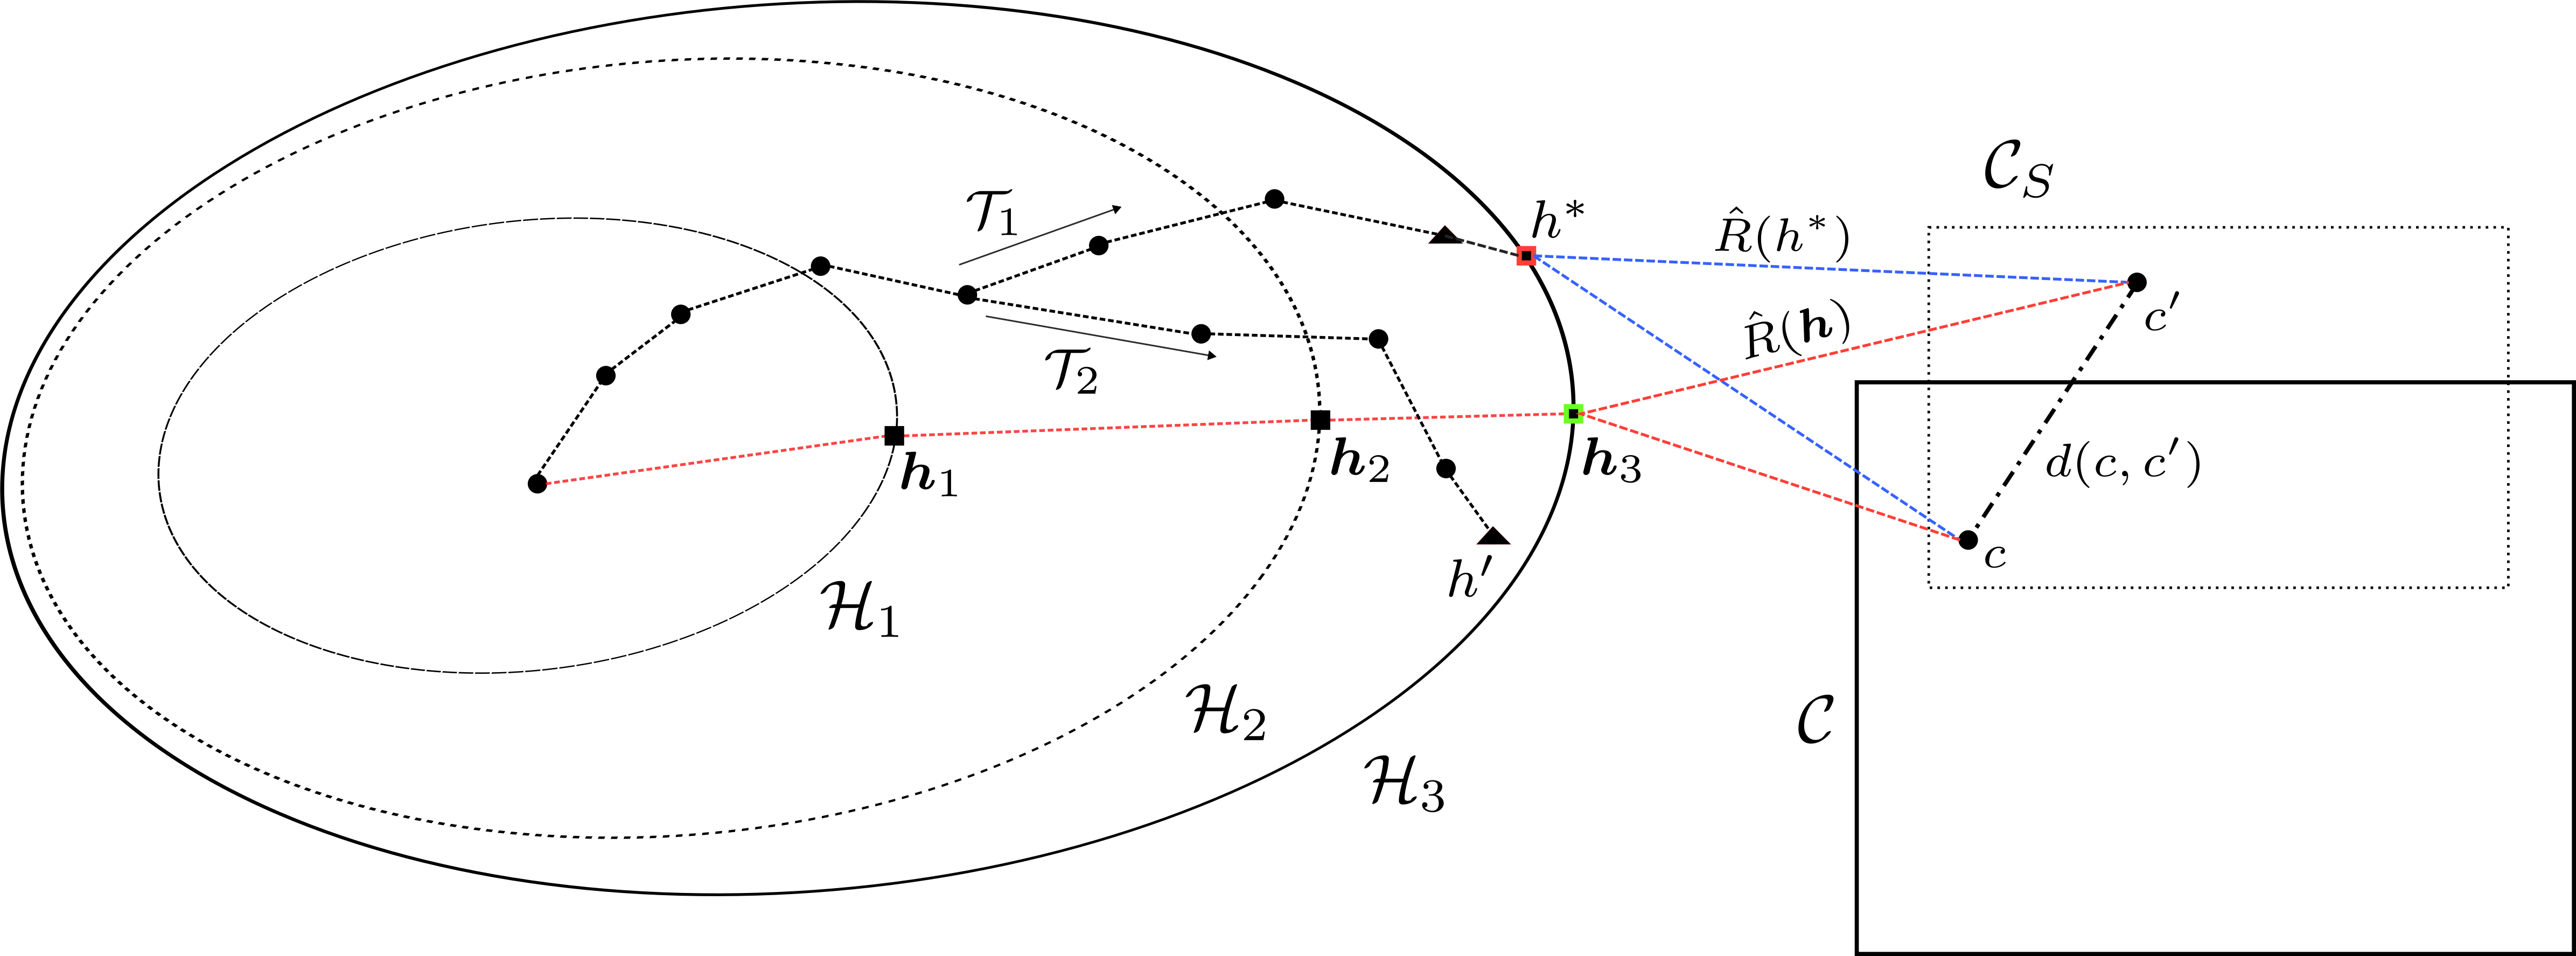
\includegraphics[width=0.7\textwidth]{media/g10.png}
  \caption{{\small \textbf{Illustrative dynamic of the learning problem.} For an incremental hypothesis space sequence $\mathcal{H}_{1},\mathcal{H}_{2},\mathcal{H}_{3}$, we aim to obtain the procedure $\mathcal{T}$ that would either reach the \textit{generalization solution} $\bm{h}$, or the \textit{empirical solution} $h^{*}$ for a particular hypothesis class, with respect to the concept $c$ and its observed concept $c'$. Model selection hence dictates how an algorithm or procedure than choose the best possible hypothesis to approximate the generalization solution from the empirical solution set. Do notice that here we explicitly state that the data would create a \textbf{proxy concept} that overlaps with the concept class and of some arbitrary `distance' from the true concept by $d(c,c')$. In case the two classes overlap, there still exists the arbitrary distance. Also, we can also observe the intuitive notion of increasing hypothesis class - while it indeed can help in getting closer to the concept class, the somewhat intrinsic property of current learning theory being the relative random procedure class make it probabilistically unstable.}}
  \label{fig:statlearnclassical}
\end{figure*}
For fixed $\mathcal{H}$, for fixed and sufficiently large $\mathcal{S}$, and no observation (data) errors, the empirical risk is the generalization risk. These two measures between $h$ and $c$ constitute the learning problem, which can also be separated into both cases - either empirical learning or generalization learning, one to minimize $\hat{R}(h)$, and one to minimize $R(h)$. Here, we emphasize such hierarchy by defining the generalization goal as the \textbf{nested criteria} for empirical risks minimization. 

\begin{definition}[Empirical learning problem]
    We present the formal form of the empirical learning. Suppose we have a \textbf{target}, $c\in\mathcal{C}$, where $\mathcal{C}$ is an arbitrary concept class that captures targets of the same type. Suppose we are provided a set of observations $\mathcal{S}$. The problem is to use certain algorithm $\mathcal{A}$ using $\mathcal{S}$, to obtain a hypothesis $h^{*}$ for a fixed $\mathcal{H}$ such that: 
    \begin{equation}\label{eq:lp1}
        R(h^{*}) = \min_{h\in\mathcal{H}} \hat{R}(h) = \min_{h\in\mathcal{H}} \underset{x\sim\mathcal{D}, x\in \mathcal{S}}{\mathbb{E}}\:\ell\{h(x),c(x)\}
    \end{equation} 
\end{definition}

The generalization best $\bm{h}$ is also called in literature as the \textit{Bayes model}, such that it reduces the Bayes risk that is the infimum of the generalization risk, $R^{*}=\inf_{h\in \mathcal{H}}R(h)$. The hypothesis $h^{*}$ is often called the \textit{empirical best}, for it being the minimal, finite hypothesis of the lowest loss evaluation on the entire observation space $\mathcal{S}$. There exists no certified assumption regarding whether $h^{*}$ aligns with the minimal generalization error.

\begin{definition}[Generalization learning problem]
    We present the formal form of the generalization learning problem. Suppose we have a \textbf{target}, $c\in\mathcal{C}$, where $\mathcal{C}$ is an arbitrary concept class that captures targets of the same type. Suppose we are provided a set of observations $\mathcal{S}$. Supposed we have an algorithm $\mathcal{A}$ that for fixed hypothesis space $\mathcal{H}$, \eqref{eq:lp1} holds true. The problem is to use certain algorithm $\mathcal{A}'$ such that, under limited availability, to obtain $\bm{h}$, satisfies: \begin{equation}
        R(\bm{h}) = \min_{h\in \mathcal{H}} R(\bm{h}) \leq \{\epsilon\}, \quad \epsilon > 0 
    \end{equation}
    For a set of risk bounds $\epsilon$. If the setting is deterministic, then there exists $\epsilon=0$ accordingly. 
\end{definition}

Then, we can partially say that generalization problem is an advancement from empirical solution. As such, empirical solution imposes the observed concept, and not the concept itself. This is reflected in modern machine learning landscape, by modelling the concept as distributions, and then using notions such as KL-divergence to measure such relative disparity. 

The process of generalization goal can be, described in certain form as the global optimization objective in which empiricism can obtain from reasonable set of assumptions and conditions. The following algorithmic framing indeed aims to focus and extradite such sense of operational goal. 

\RestyleAlgo{ruled}
\SetKwComment{Comment}{}{}
\SetKwBlock{Objective}{Objective}{}
\begin{algorithm}[htb]
    \renewcommand{\algorithmcfname}{Optimization problem}
    \caption{Empirical-generalization learning dynamics (non-proxy)}
    \KwData{$(x_{i},y_{i})\in\mathcal{S}, \Gamma \supset \mathcal{S}$, objective $\ell(y,f(x))$, $\nabla(\cdot)$ differentiable gradient field on $\ell$.}
    \KwResult{Expected optimized model to the minimal error on the objective $\ell(\cdot,\cdot)$, dependent on $\mathcal{S}$.}
    \Begin
    {
        $\Gamma\supset \mathcal{S}$, the general set\;
        $R(\cdot),\hat{R}(\cdot)\gets\ell$ as objective functional\;
        \For{Fixed $\mathcal{H}$, with $h\in\mathcal{H}$, for $\epsilon > 0$}{
            Find $h\to \bm{h}'$, using algorithm $\mathcal{A}$ for minimization objective, such that 
            \begin{equation}
                \mathcal{A}\left(\min_{h\in\mathcal{H}} \hat{R}_{\mathcal{S}}(h) + R(h)\right) \leq \epsilon 
            \end{equation}for procedure $\mathcal{A}(\cdot,\cdot)$ of structural constraints.\;
        }
    }
    \Return{Optimized model $h$ on arbitrary objective space $(\ell,\nabla)$.}
    \label{algo:algo_optim_ideal}
\end{algorithm}

These two stages of learning procedure comes of as the intrinsic design of machine learning setting. As opposed to interpolation, where empirical learning problem would have to be put into first priority to achieve the best possible point-through model, machine learning leans on approximation more and a separated criterion that is only visible in the learning setting - the fact that we are using $c'$ to extract $c$. This disparity is exactly the \textbf{generalization problem}, of which is then also the goal of machine learning, to approximate the general solution using the observed solution. One then can ask what is the difference between the two notions, and when we can guarantee that both will `converge' to the same point. The process of \textbf{model selection} is then the procedure that will optimize $h\in \mathcal{H}$ to a given target fixture, such as the empirical best. 

One of the major assumption or observation from the point of the hypothesis class, is that the hypothesis cannot know the generalization error. Thereby, the more efficient and often used procedure/algorithm in training, is then the \textit{empirical risk minimization} (ERM) method, minimizing only the empirical risk to the empirical best; then, certain measures to `generalize' this heuristically is apprehended on the hypothesis. The process of model selection is also the place that we get the concept of \textbf{bias-variance tradeoff}, and its longstanding form to be a foundational metric on model selection. 

\subsection{Overfitting and underfitting}

Following the above framework of statistical probabilistic learning theory, one understanding about the concept of underfitting and overfitting (similar to \cite{James2021}) can be reached, using the notion of \textit{partitioning} of observation space. Such work is typically done because of \textbf{practical condition}, in which the following constraints is applied.
\begin{assumption}\label{assume:cpi_transparency}
    No knowledge of $c\in\mathcal{C}$ is provided. \footnote{Few points need to be said about this assumption. This assumption represents the \textit{worst-case possible} of a system dynamic. From the perspective of a designer, inherent leakage of information can be provided in the design of a model. In such, case we are operating in the mode of a \textit{resource-constrained, closed} game, in which the model with further assumptions of fixed class, operates on. The problem space itself is inherently large and penalize any additional structural changes. If one is to occur, we usually mention it as \textit{implicit bias}, but another name that would be more fitting would be \textit{structural attractor}, after the notion of gradient attractor in chaotic systems.}
\end{assumption}

Without such knowledge, $R(h)$ cannot be computed, accordingly. We specify such approach as \textit{heuristic}, as it is only an approximation, and for better definition, we define it as followed. 

\begin{definition}[Heuristic empirical risk]
  Given a dataset $\mathcal{S}$ of size $m$, supposedly of the concept $c\in \mathcal{C}$, and the hypothesis $h\in \mathcal{H}$, then the \textbf{heuristic empirical risk} take a partitioning $k<m$ with $k/m\geq 1/2$, hence defining the heuristic empirical loss on $k$, denoted $\hat{R}_{k}(h)$. 
\end{definition}

\begin{definition}[Heuristical generalization risk]
  Given a dataset $\mathcal{S}$ of size $m$, supposedly of the concept $c\in \mathcal{C}$, and the hypothesis $h\in \mathcal{H}$. Fixed $\hat{R}_{k}(h)$, for the final optimization of algorithm $\mathcal{A}$, then the \textbf{heuristic generalization risk} take the remaining 2-partition of portion $p=k-m$, hence defining the heuristic generalization loss on $p$, denoted $\hat{R}_{p}(h_{\mathcal{A}})$. 
\end{definition}
The two heuristic definition however, can be noted to not be equal to the true generalization risk - empirical risk pair in reality. Nevertheless, one can then define overfitting and underfitting in such manner. 
\begin{definition}[Underfitting]
  A model $h$ is called \textbf{underfitting} if for a constant $\epsilon > 0$ chosen for the setting, then $\hat{R}_{k}(h_{\mathcal{A}})>\epsilon$, $\hat{R}_{p}(h_{\alpha})> \epsilon$ over the entire observation space. 
\end{definition}
Usually, underfitting is defined to be such that test error is smaller than training error partition, however, we do not think that is a good definition. Especially since, at least in this setting, the empirical error under algorithm $\mathcal{A}$ is reduced to the representative smallest error that $\mathcal{A}$ can achieve on that particular model, within particular setting of $h$, then come the heuristic generalization error. Considering also that $k/m\geq 1/2$, that is, at least the training partition is half of the observation set, then only under very specific case will $\hat{R}_{p}(h_{\alpha})$ be smaller than $\hat{R}_{k}(h)$, statistically speaking. Thence this line of thought also reinforces the idea that both of them will be larger than the threshold $\epsilon$. Usually, heuristically, this threshold of error is $0.3$, normalized. Next, we define the notion of overfitting. 

\begin{definition}[Overfitting]
  A model $h$ is called \textbf{overfitting} if there exists a specific constant $\epsilon>0$ chosen for the setting, such that $\hat{R}_{k}(h)<\epsilon$, $\hat{R}_{p}(h_{\alpha})> \epsilon$ over the entire observation space.
\end{definition}
Namely, this mean that the static learning makes the generalization error worse. This draws the analogy of the student - studying explicitly for the past paper tests, yet unaware of the larger margin of questions in the large set of the test paper pool, leading to subpar performance. Similarly, overfitting is theorized to be fitting too fit to the reduced observation space - hence when it comes to the generalization observation space, it fails within such heuristic. The notion works on the mask of the risks, $\hat{R}_{k}$ and $\hat{R}_{p}(h_{\alpha})$. 

In practice, Assumption~\ref{assume:cpi_transparency} means we cannot have $c\in\mathcal{C}$, or its probabilistic interpretation $\mathcal{D}$ such that $x\sim\mathcal{D}$, or in the extreme non-structured case, $(x,y)\sim \mathcal{D}$. In such case, the typical practical fix relies on the partitioning of the available partitioning space, that is, the empirical-generalization proxy. For large enough singleton count of $|\{(X_{k},Y_{k})\}|$, we assume that $\hat{R}_{\mathsf{Gen}}(h)\approx R(h)$. Thus, the algorithm can be stated in a form as Algorithm~\ref{algo:algo_optim_no_c}.

\RestyleAlgo{ruled}
\SetKwComment{Comment}{}{}
\SetKwBlock{Objective}{Objective}{}
\begin{algorithm}[htb]
    \renewcommand{\algorithmcfname}{Optimization problem}
    \caption{Empirical-generalization learning dynamics (proxy)}
    \KwData{$(x_{i},y_{i})\in\mathcal{S}, y_{i}=\{\pm 1\}$, hinge objective $\ell(y,f(x))$, $\nabla(\cdot)$ differentiable gradient field on $\ell$.}
    \KwResult{Expected optimized model to the minimal error on the objective $\ell(\cdot,\cdot)$, dependent on $\mathcal{S}$.}
    \Begin
    {
        $((X_{1},Y_{1}),\dots)_{n}\gets\mathsf{Partition}_{n}(\mathcal{S})$\;
        $\{(X_{j},Y_{j})\}\gets \mathsf{Train}$\;
        $\{(X_{k},Y_{k})\}\gets \mathsf{Gen}$ for $k\ne j$\;
        \For{Fixed $\mathcal{H}$, with $h\in\mathcal{H}$, for $\epsilon > 0$}{
            (Optimistically) achieve $h\to \bm{h}'$, using algorithm $\mathcal{A}$ for minimization objective, such that 
            \begin{equation}
                \mathcal{A}\left(\min_{h\in\mathcal{H}} \hat{R}_{\mathsf{Train}}(h) + \hat{R}_{\mathsf{Gen}}(h)\right) \leq \epsilon 
            \end{equation}for procedure $\mathcal{A}(\cdot,\cdot)$ of structural constraints.\;
        }
    }
    \Return{Optimized model $h_{\mathcal{A}}$ on arbitrary objective space $(\ell,\nabla)$.}
    \label{algo:algo_optim_no_c}
\end{algorithm}
The assumption above of the generalization set to the generalization truth error is apparent in the usual system theorem, Theorem~\ref{thm:minimalNeu}.
\begin{theorem}[\cite{10.5555/2371238}]\label{thm:minimalNeu}
    For fixed $\mathcal{H}$, for fixed and sufficiently large $\mathcal{S}$, and no observation errors, the empirical risk is the generalization risk: \begin{equation}
        \underset{\mathcal{S}\sim \mathcal{D}^{m}}{\mathbb{E}}[\hat{R}_{\mathcal{S}}(h)]  = R(h)
    \end{equation} 
\end{theorem}

\begin{proof}
    By linearity of the expectation, and the fact that we assume the sample is given i.i.d., we can write: 
\begin{equation}
    \begin{split}
        \underset{S \sim \mathcal{D}^m}{\mathbb{E}}[\hat{R}_S(h)] 
        &= \frac{1}{m} \sum_{i=1}^m 
            \underset{S \sim \mathcal{D}^m}{\mathbb{E}} 
                    \left[ \mathbbm{1}_{h(x_i) \ne c(x_i)} \right] \\
        &= \frac{1}{m} \sum_{i=1}^m 
            \underset{S \sim \mathcal{D}^m}{\mathbb{E}} 
                \left[ \mathbbm{1}_{h(x) \ne c(x)} \right], \\
    \end{split}
\end{equation}
for any \( x \) in sample \( S \). Thus, we result in

\begin{equation}
    \begin{split}
        \underset{S \sim \mathcal{D}^m}{\mathbb{E}}[\hat{R}_S(h)] 
            &= \underset{S \sim \mathcal{D}^m}{\mathbb{E}} 
            \left[ \mathbbm{1}_{h(x) \ne c(x)} \right] \\
            &= \underset{x \sim \mathcal{D}}{\mathbb{E}} 
            \left[ \mathbbm{1}_{h(x) \ne c(x)} \right] \\
            &= R(h).
    \end{split}
\end{equation}
which yields the desired result. 
\end{proof}

This theorem can be transferred to a more generalized conjecture, of which fit the generalized notion of the empirical proxy and so on. 
\begin{conjecture}
    Supposed $\mathcal{H},\mathcal{C}$ are fixed, for $\mathcal{S}$ is the empirical $c^{*}$ for $c\in \mathcal{C}$ the true concept. Then, for algorithm $\mathcal{A}(\cdot,\cdot)$ enforcing minimization apparatus, and the specific objective on the second argument, we have:
    \begin{equation}
        \begin{split}
            &\underset{j\to\infty,\mathcal{S}_{i}\neq\mathcal{S}_{k}}{\mathcal{A}}\left(\min_{h\in\mathcal{H}} \hat{R}_{\mathsf{Train}}(h) + \hat{R}_{\mathsf{Gen}}(h), [\ell]\right)\\
            & \quad \quad \approx \mathcal{A}\left(\min_{h\in\mathcal{H}} \hat{R}_{\mathcal{S}}(h) + R(h), [\ell]\right) + \epsilon_{\mathcal{S}}
        \end{split}
    \end{equation}
    For $\mathcal{S}_{i}\neq\mathcal{S}_{j}$ such that there are only distinct samples, $j$ the observation set size, $[\ell]$ the set of structural or empirical objectives enforced on the problem landscape, and $\epsilon_{\mathcal{S}}$ is the empirical minimum that the algorithm result can achieve assuming sufficient `perfect interpolation'. 
\end{conjecture}

By the end of this section, we would also want to note that we deliberately choose an expression basis of $\mathcal{A}$ via the couple tuplet $(\min, [\ell])$ as a choice for \textit{algorithm-agnostic class} of algorithm satisfies the dynamic only, not just implementations. The algorithm, in certain sense, depends much more on structural assumptions, of which is not accessible via observations but via design, and intrinsic information specified in the observation class itself. This is a requirement for fine-tuning analysis in the long-run, as there exists a myriad of different approaches. Indeed, the classical theory of learning simply does not have much to offer in terms of a unified perspective, in which important factors are analysed of its realization. Specifically speaking of such, classical theory does do worse in many parts, for example, the aspect of transparency given the model, supervisor and the concept, of which their roles are not fully understood or formulated correctly, both in controlled setting and extension to replication of real life examples. Thereby, the problem requires a newer theory of learning to come forward. A new learning theory must extend beyond what constitute the basic learning model, such as the idealized PAC-learning, and statistical learning setting in general. More specifically, we want to design a learning theory that is more akin to \textbf{modelling theory} of its internalization, but also attain the learning of machine learning theory. 

Within the constraints of such theoretical framing, we can then construct a different notion in which the generalization and the empirical learning problem can possibly relate to each other, at least from the statistical framework. Let us consider the problem of mathematical modelling in such sense. Beside the model class construction, which will be discussed in further sections, the entire idea of this structuralization is to refine the framework of which learning and so on can be defined itself. 

\section{System-wide structuralization}

From which we can draw out of the above discussions, concurrent theories are inherently unstable and with many variations, making them ill-suited for instant application on analysis of different models without losing major information about the structural details and expressions. Hence, we propose a novel analysis on the basis of the axiomatization of the learning setting, under various structural assumptions, which lies in the implementation sections. For now, we defer to the insight in which justify such movements. 

\subsection{The idea of neural network formalism}
Previously, we have been discovering, examining past results and testing on models of different types, generally classical models. While decisive, each modelling setting requires different analysis and is often not so streamline, typically fragmented as per different functional schemes, probabilistic schemes, optimization and algorithmic-based choice of designs, and so on. They have barely any unified view or general patterns for extension, thus making analysis inherently difficult. Within such, our interest, and discovery, posit that the formalism or the idea of neural network (accordance to designs and patterns of \cite{mcculloch_pitts_1943,hebb_1949,rosenblatt_1958,widrow_hoff_1960_adaline,minsky_papert_1969,fukushima_1980,kohonen_1982,hopfield_1982,werbos_1974,rumelhart_hinton_williams_1986,cybenko_1989,hornik_1991,hochreiter_schmidhuber_1997,lecun_bottou_bengio_haffner_1998,bishop_1995,haykin_1994}) and some of its modern understanding (as of \cite{goodfellow2016deep,zhang2023mathematical,hinton_osindero_teh_2006,lecun_bengio_hinton_2015,goodfellow_et_al_2014,srivastava_hinton_2014_dropout,szegedy_2014_inception,simonyan_zisserman_2014_vgg,vaswani_et_al_2017_transformer,he_zhang_ren_sun_2016_resnet,devlin_2018_bert,brown_et_al_2020_gpt3}) practiced and exhibited, to be, in its general form, the correct but ill-defined and poorly developed framework. Thus is our goal in this section to layout such task, and the development that will be described in this section. 

\subsubsection{Basic understanding}

In modern form, a neural network (\cite{goodfellow2016deep,zhang2023mathematical}) $N$ is typically specified by the dual $(L,[S])$ where $L$ is the number of processing layer of a neuron, and $[S]$ is the list of neurons configuration per layer - for example, the number of neurons per layer, and so on. For such network, the definition can be simple as followed 

\begin{definition}[Standard multilayer network, \cite{zhang2023mathematical}]
    We define a $K$-layer fully-connected deep neural network with real-valued output. Let $m^{(0)}=d$ and $m^{(K)}=1$ for $m$ the width of the network, and $d$ the shape of the input vector. We then recursively define: 
\begin{align}
    x_{j}^{(0)} &= x_{j} \quad (j=1,\dots,m^{(0)}),\\ 
    x_{j}^{(k)} &= h\left(\sum^{m^{(k-1)}}_{j'=1} \theta_{j,j'}^{(k)}x_{j'}^{(k-1)}+ b_{j}^{(k)}\right)\quad (j=1,\dots,m^{(k)}),\\
    f(x) & = x_{1}^{(K)} = \sum^{m^{(K-1)}}_{j=1} u_{j}x_{j}^{(K-1)}
\end{align}
where $k = 1,2,\dots,K-1$, for the model parameters can be represented by $w=\{[u_{j}, \theta_{j,j'}^{(k)}, b_{j}^{(k)}]: j,j',k\}$ with $m^{(k)}$ being the number of hidden units at layer $k$; $\theta\in \mathbb{R}^{m}$ the weight of the neuron.
\end{definition}

Here, each neuron is denoted by their expression as $f(\mathbf{W}^{\top}\mathbf{x}+b)$ for the activation function $f$. We can simplify a lot of those structures above into the neural network schemes. For example, the linear function class case can be simplified to a single $(2,[n,1])$ neural network, such as: 
\begin{align}
    x^{(0)}_{j} &= x_{j} \quad (j=1,\dots,n)\\
    x^{(1)} &= \sum_{j'=1}^{n} w_{j'}x_{j'}, 
\end{align}
without the activation function $h$. The polynomial neural network can be represented by simply a shallow, $[3,p]$ neural network. More concretely, if we take the \textit{input channel} as a (pre-)layer, then
\begin{align}
    x_{j}^{(0)} &= x_{j} \quad (j=1,\dots,m^{(0)}),\\ 
    x_{j}^{(1)} &= h\left(\sum^{m^{(0)}}_{j'=1} \theta_{j,j'}^{(1)}x_{j'}^{(0)} \right)+b_{j}^{(k)}\quad (j=1,\dots,m^{(1)}),\quad h(x_{j})=x^{j}\\
    f(x) & = x_{1}^{(2)} = \sum^{m^{(1)}}_{j=1} u_{j}x_{j}^{(1)}
\end{align}
for a neural network of shape $(3,[n,n,1])$, and of polynomial custom scaling function. For support vector machine, this is even harder to do, since its definition varies between different notion of the model itself. However, it is interesting because we can treat it as an arbitrary generation of a neural network structure. There are papers about formalizing SVM in the sense of neural network, including making it to be an infinitely-wide shallow neural network, for example, \cite{chen2021equivalence,wang2019svmdsn,zhang2014equivalence}, however, the structure that is formed from the SVM learner can be expressed as followed:

\begin{setting}[Support vector machine]
    For any given optimization problem on input space $x_{i}\in \mathbb{R}^{d}$, and label $y_{i}=\{\pm 1\}$, the shallow neural network resultant from the training procedure is always of the form:
    \begin{align}
        x_{j}^{(0)} &= x_{j} \quad (j=1,\dots,m^{(0)}),\\ 
        x_{j}^{(1)} &= \sum_{j'\in m^{(1)}} \theta^{(1)}x_{j'}^{(0)}K(x_{j'}^{(0)},x)\\
        f(x) & = \sign{(x_{1}^{(2)}) }
    \end{align}
    for a specific kernel $K(x,x')$. 
\end{setting}

Those three fundamental conversions to neural network raise interesting insight into the neural network formalism. For linear and polynomial shallow neural network, we design the network and then provide it with a training scenario, evaluated of the proxy generalization. SVM however can be considered an adaptive data construction, where the neural network is constructed from the dataset or observation set itself, using minimization on RKHS and with constraints. This prompts exactly as such, on one side the pre-optimization construction, and one is the post-construction optimization of a neural network architecture. This interpretation is surprisingly useful when talking about neural network's unit-like structure. Hence, from such evidence prompts us to analyse a neural network, not in only the sense of managing its layers, but also by its unit components together. 

This way of analysing unit-wise gives us much more interpretability, and also potential for a newer kind of network specification. As far as we are concerned of, a neural network can represent an active \textit{mathematical modelling system}. This then indicates, for example in adversarial learning case between the target neural network tailored to specific concept, and the learning hypothesis network, then the process of learning itself can be loosely interpreted as a concept of mathematical modelling representation learning, even in the case of black-box model, and not just simply phenomenological modelling of statistical data. To do this, we will examine the structure from the perspective of a \textbf{generator}.

\subsubsection{The SVM generator}

Support vector machine, first formally originated from \cite{Vapnik1999-VAPTNO}, is a model inherently, specifically defined for pattern recognition task, and binary classification via an \textit{optimal separating hyperplane}. There are two variants for SVM, namely, for linear and nonlinear hyperplane, but the main general aspect of SVM is its reversal of the direction on model building - instead, it aims to minimize the structure of a model, using the data-dependent structure, or \textit{support vectors}. 

The SV machine implements the following two precursor ideas: It maps the input vectors $x$, supposed of the setting, into a high-dimensional feature space $Z$ through some nonlinear mapping, chosen a priori. In this space, an optimal separating hyperplane is constructed. By statistical learning theory, Vapnik restricted the function class (as for infinite hypothesis it is impossible to learn) to the class of hyperplanes by 
\begin{equation}
    \langle \mathbf{w}\cdot \mathbf{x} \rangle + b = 0 ; \quad \mathbf{w}\in \mathbb{R}^{n} , b\in \mathbb{R}
\end{equation}
which $\mathbf{w}$ is the controlling weight, $\mathbf{x}$ is the input space to the space of all binary $\{-1,+1\}$ category. Hence, this basically divide the input space into two: one part containing vectors of the class $-1$ and the others being $+1$. If there exists such a thing, then it is said to be \textit{linearly separable}. To find the class of a particular vector $\mathbf{x}$, we use the following decision function 
\begin{equation}
    f(\mathbf{x}) = \mathrm{sgn}[\langle \mathbf{w}\cdot \mathbf{x}\rangle+ b]
\end{equation}
This is called the \textbf{hyperplane classifier} class\footnote{As can be understood simply from such, there exists many hyperplanes that can correctly classifies the classes. It has been then shown that the hyperplane that guarantees the best generalization problem performances is the one with the maximal margin of separation between two classes (\cite{Cristianini2000AnIT}).}. The above form of finding final classification can then be presented in dual form, which then depends only on dot products between vectors, as 
\begin{equation}
    f(\mathbf{x}) = \mathrm{sgn}\left(\sum^{\ell}_{i=1} y_{i}\alpha_{i} \langle \mathbf{x}\cdot \mathbf{x}_{i} \rangle+ b\right)
\end{equation} 

where $\alpha_{i}\in \mathbb{R}$ is a real-valued variable that can be viewed as a \textit{measure} of how much informational value $\mathbf{x}_{i}$ has (for $x_{i}$ the support vectors we get from training)\footnote{The \textit{support vector} of a particular hyperplane $\mathbf{y}$ is the collections of all points that lies closest to the hyperplane, which is specified as condition for maximization on both side of maximal margin vector machine.} The second idea is of the \textit{kernel method}. This particular method, useful and well-known of the time SVM was created, gain a more prominent position among other techniques, including neural network. Specifically, this method is characterized by the mapping of the input vectors into a richer (usually high-dimensional) feature space where they satisfy \textit{linear separable} criteria. This prompted the possibility to solve nonlinear problem through such mapping, and indeed yields a nonlinear decision surface in the input space, which is linear in the feature space. A \textbf{kernel} (function) is then a function $k(\mathbf{x},\mathbf{y})$ that given two vectors in input space, return the dot product of their images in feature space such that $k(\mathbf{x},\mathbf{y})=\langle \phi(x), \phi(y) \rangle$ for the nonlinear mapping $\phi$. The general form of SVM is then usually cited as 

\begin{equation}
    f(\mathbf{x}) = \mathrm{sgn} \left(\sum^{\ell}_{i=1} y_{i}\alpha_{i}k\langle \mathbf{x}\cdot \mathbf{x}_{i} \rangle\right)\quad \ell \leq n
\end{equation}
for any particular final categorization. One of the major problem for analysing SVM, is in the properties of it potentially having infinitely many parameters, depends on the size of the dataset. This makes the curve of both bias-variance and double descent not applicable in such regard - infinitely many parameters' complexity, yet still finite complexity class\footnote{From such observation, it would seem imperative that the notion of complexity based solely on the parameter counts of certain model construction is ill-equipped for certain flavours of machine learning model, in this case support vector machine (in the same type is the Gaussian Mixture Model). No double descent has been observed by empirical reports record per the author's knowledge.}. 

With respect to the observable space, SVM and neural network, we can call the construction scheme of SVM a type of \textit{backward construction} from data $\mathcal{S}$. Or rather, the following algorithm represents SVM construction problem: 

\RestyleAlgo{ruled}
\SetKwComment{Comment}{}{}
\SetKwBlock{Objective}{Objective}{}
\begin{algorithm}[htb]
    \renewcommand{\algorithmcfname}{Factory}
    \caption{Support Vector Machine - backward construction.}
    \KwData{$(x_{i},y_{i})\in\mathcal{S}, y_{i}=\{\pm 1\}$, hinge objective $\ell(y,f(x))$, $\nabla(\cdot)$ differentiable gradient field on $\ell$.}
    \KwResult{Expected optimized model to the minimal error on the objective $\ell(\cdot,\cdot)$, dependent on $\mathcal{S}$.}
    \Begin
    {
        $d\gets \dim|\mathcal{S}|$\;
        $n\gets|\mathcal{S}|$\;
        $\ell(y,f(x))=\max(0,1-yf(x))$\;
        Kernalization $\phi:\mathbf{x}\to\mathbf{x}'$\;
        $f(\mathbf{x})\gets \mathbf{w}^{\top}\phi(\mathbf{x})+b$\;
        \Objective
        {
            Attain the minimization 
            \begin{equation}
                \min_{w,b\in f} \frac{1}{2}||w||^{2} + C \sum_{1\leq i\leq n}\ell(y_{i},f(x_{i}))
            \end{equation}
            Ideally for $y_{i}(\mathbf{w}^{\top}\phi(\mathbf{x}_i)+b)\geq 1, \: \forall i, y_{i}\in\mathcal{S}$, penalized by $\ell$.\;
        }
    }
    \Return{Optimized model $\mathsf{SVM}(f)$ on objective $\ell$ of $\nabla$ field.}
    \label{algo:algo_SVM_no_kernel}
\end{algorithm}

Such a factory is reversed inherently, and with its formulation constrained in the form $\mathbf{w}^{\top}\phi(\mathbf{x})+b$, of which is equivalent to a non-linear shallow neural network with infinite width (\cite{wang2017research,chen2021equivalence}), but is not a full-fledged neural network in technicality, hence it is only a functional equivalence. That is, such result only indicates that for $N\to \infty$ of the number of neurons of a single-hidden layer neural network, $\sum_{j=1}^{N}a_{j}(w_{j}^{\top}x+b_{j})$, then 
\begin{equation}
    \mathsf{NN}(x) \approx \mathsf{SVM}(x) = \sum^{\ell}_{i}\alpha_{i}k\langle x,x_{i}\rangle, \ell \leq n
\end{equation}
The support vector, $\ell$ list, is inherently implicit of the factory itself. On the other hand, typical deep learning or neural network constructions are rather \textit{forward-constructed}, that is, the model is in a sense, prefabricated then tested of its efficacy, and thus the effective performance of the model is limited by iterations of its restricted frame. We can easily visualize the factory of which neural network are constructed, different of the SVM factory case:

\section{Complexity notion}

Assume the working space is the real field $\mathbb{R}^{n}$. Let us recall a model $h\in\mathcal{H}$ of certain hypothesis class $\mathcal{H}$. Then, the \textbf{complexity} refers to the complexity of the hypothesis $h$ itself; there is also the notion of class maximal complexity for $\mathcal{H}$. Complexity in this case refers to the mass of the model, or rather, to answer the following questions:
\begin{enumerate}
    \item What is the effective expression range of a hypothesis?
    \item What is the hypothesis structured in?
    \item If the model is constructed by parameters, how many parameters are there?
    \item How many components are there in specific model $h$, and how would another model $h'\in \mathcal{H}$ differs from $h$?
\end{enumerate}

Those questions are not so easily answered. Specifically, analysis often puts the hypothesis class $\mathcal{H}$ as a class of functions. So, there exists the class $\mathcal{H}_{n}$ of $n$-th degree polynomials, or else. Effective complexity in such case means the range of expression a function can give - for example, for $n$-th polynomial class. For the class $\mathcal{H}_n$ of polynomials of degree $n$ on a closed interval $[a,b]\subset \mathbb{R}$, the Weierstrass approximation theorem guarantees that, as $n\to \infty$, any continuous function $f:[a,b]\to \mathbb{R}$ can be approximated arbitrarily closely in the uniform norm. Hence, the expressive complexity of $\mathcal{H}_n$ grows with $n$, but for fixed $n$ only a finite-dimensional subset of $C([a,b])$ is exactly representable. This distinction highlights the difference between \emph{approximation capacity} of a hypothesis class and the \emph{exact representational capacity} captured by its parameterization. These expressions depend on the field or space the hypothesis class lives in, for example, if the hypothesis is configured to work in the set of all functions in $\mathbb{F}=\mathbb{R}$ of algebraic field, then we call it the algebraic family. There are various hypothesis classes in such case, and usually, not a lot of them can be analysed and represented in the same way, and hence also the analysis of the `size' of the hypothesis, also between different hypothesis classes, prompted the usage of a more general notion, called \textbf{representation complexity}\footnote{Representation complexity refers to the number of components needed to express $h$ and generally, any hypothesis in $\mathcal{H}$. This is often the parameters count, since the parameters themselves are used in constructing the function in algebraic system. Thus, again, an $n$-th degree polynomial might have $2(n+1)$ parameters, for $n+1$ variational input (or variable), and $n+1$ coefficients. Notice that we specifically at the beginning, use the notion of algebraic structure $\mathbb{R}$ because of it. If we restrict ourselves to the expression, for example, for $\mathbb{B}=\{0,1\}$, then it can be expressed in various ways in logic theory, such as conjunctive normal form (CNF), disjunctive normal form (DNF), and else. This forbid the analysis based on the effective process itself, but rather the number of components required, hence taking them as complexity of construction.}.

\begin{table*}[htb]
  \centering
  \footnotesize
  \begin{threeparttable}
    \caption{Descriptions of complexity measures applied to models and learning processes, from \cite{STL_Hajek_Maxim_2021,10.5555/2930837,10.5555/2371238,10.5555/200548} and \cite{Vapnik1999-VAPTNO} with some custom notions.}
    \label{tab:polynomial_test}
    % three columns: adaptive widths
    \begin{tabularx}{\textwidth}{ L{0.15\textwidth}
                                     L{0.1\textwidth} 
                                     L{0.4\textwidth}
                                     >{\RaggedRight\arraybackslash}X }
      \toprule
      \textbf{Type} & \textbf{Notation} & \textbf{Purposes} & \textbf{Notes} \\
      \midrule
      Representation
        & $\mathcal{M}_{r}$ 
        & Complexity of encoding a model (size of representation, alphabet-dependent).
        & Model-level measure. \\
      \addlinespace[1pt]
      Expressive 
        & $\mathcal{M}_{e}$
        & Complexity of the model's observable behaviour (operational expressivity of the mapping it implements). 
        & Model-level measure.\\
      \addlinespace[1pt]
      Structural
        & $\mathcal{M}_{s}$
        & Complexity of the model's internal architecture (how components compose and interact).
        & Model-level measure.\\
      \addlinespace[1pt]
      Structural mass
        & $\mathcal{M}_{\Sigma}$
        & Aggregate representation size derived from representation complexity across the model.
        & Sum of $\mathcal{M}_{r},\mathcal{M}_{e},\mathcal{M}_{s}$\\
      \addlinespace[1pt]
      Sample
        & $\mathcal{M}_{p\in\mathcal{S}},\mathcal{M}_{p}$
        & Number of samples required to reach a prescribed performance level (statistical sample-count).
        &Process-level measure.\\
      \addlinespace[1pt]
      Sample space
        & $\mathcal{M}_{\mathcal{S}}$
        & Intrinsic complexity of the data distribution / sample domain (richness, diversity, structured-ness).
        & Global process measure.\\
      \addlinespace[1pt]
      Optimization
        & $\mathcal{M}_{\epsilon}$
        & Complexity of the learning algorithm (convergence rate, computational/iteration cost, sensitivity) or worst-medium-best learning cost. 
        & Process-level measure.\\
      \addlinespace[1pt]
      \bottomrule
    \end{tabularx}

    \begin{tablenotes}
      \footnotesize
      \item[] \textbf{Notes:} The notion of structural mass is convoluted. In certain setting, it is simply the parameter space $\theta\in\Theta$, but in some setting, there exists fundamental difference than identically weighted parameter space complexity, as seen in multi-basis polynomial models, not taking into account homogeneous deep learning networks. Optimization complexity coincides with PAC-learning bounds for polynomial runtime, and \textit{sample complexity} sometimes can only be the dimension of the input/observation space.
    \end{tablenotes}
  \end{threeparttable}
\end{table*}

The above complexity (and so is in Table~\ref{tab:polynomial_test}), aside from sample space-related measure, can also be applied onto the concept class's members itself. We also take the class complexity in such case, as the argument that maximize those measure: that is, the largest value of the measure, taken on the class as the class's complexity.\footnote{Expressive complexity measures the variety of input-output behaviours the model can implement.}\footnote{Structural complexity is decomposable into component-wise measures (e.g., per-layer, per-module) and useful for architectural comparisons.}\footnote{Sample complexity depends on hypothesis class, loss, and desired error/confidence. Further clarification must be made of a grounded definition for utilization.}\footnote{Sample space complexity infers the statistical measure over the sample space; affects learnability and effective sample size.}\footnote{We also note that the notion of optimization is usually hard to pin down analytically, often characterized empirically or by worst-case bounds.}

The next complexity measures that can be taken of, comes from the learning process structure itself. Usually, in statistical learning theory (\cite{STL_Hajek_Maxim_2021,10.5555/2371238,10.5555/2621980}), we often use the setting that is related to \textbf{supervised process}. This usually means the process can be configured in a feedback loop, or induced response toward the model - often come from the observational space, where the concept that is set to be the target of the process - then called as learning process - is conjured. For now, we reserve this to the classical learning theory and process, and will not inquire further of such direction. 

The learning process assumes an operational space containing the structure, for example, $\mathbb{R}$-encoding space of real values, and a set of \textbf{samples} living in such space, denoted $\mathcal{S}$. Those samples are often referred to as the \textbf{observation set} of a particular objective of learning. As mentioned above, $\mathcal{S}$ belongs to the concept $c$, assumed to be of certain concept class $\mathcal{C}$. $\mathcal{S}$ is obtained by using an observing process to create or generate the result. This process can be determined or considered in multiple way, however, generally can be considered by having a deterministic interpretation (using an explicit function $c(x)$) or by probabilistic approach (modelling a distribution $\mathcal{D}$). Hence, we gain another type of complexity, with regard to the process called \textbf{sample complexity} - usually defined of cardinality - the amount of sample needed for particular purpose, for particular objective. For the complexity category up to the structure of the learning setting by itself, we call it the \textbf{sample space complexity}. 

One final complexity that is worth mentioning is then the \textbf{optimization complexity}, measure on the action of the learning algorithm. By such, it investigates the construction of an optimization algorithm solely dependent on its size of the algorithm, and other non-process related measures. Optimization complexity can also be related or expressed, in situation of time complexity, which is typical in computing system. 

One might ask why we need to determine and categorize complexity measures and the need to generalize and differentiate of each one. Indeed, while in usual use cases, such complexity notion can be considered sufficient in controlling and gauging the model itself. However, just as \cite{James2021} indicated in the section on deep learning double descent, such complexity might eventually, of some regions, inadequate to express and evaluate the complexity of the model in its operations any more. Such transition is unanswered, and while the founding of complexity notion is still fragmented, it is indeed difficult to not paying attention specifically to those notions themselves. Considering such of the learning framework and the more sophisticated goal that we push forth of reforming the learning theory, it is then natural to define such. 

\section{Attractor-based insights}

The above reformulation in this chapter, giving insights of the learning formulation typically observed, arguably still attains a lot of assumptions, of which we settle for the next section. Optimization procedure~\ref{algo:algo_optim_ideal} and procedure~\ref{algo:algo_optim_no_c} define the precursor tradeoff in the problem space, or rather, the heuristic-generalization tradeoff. We can state it as the following to clarify such problem in plain sight. 

\begin{theorem}[Heuristic-generalization tradeoff, model selection]
    An algorithm $\mathcal{A}$ on the system $(\mathcal{H},\mathcal{C},\mathcal{A})$, for the expected empirical heuristic $\hat{R}_{\mathsf{Train}}(h)$ and generalization heuristic $\hat{R}_{\mathsf{Gen}}(h)$ on $\mathcal{S}$, on the measure landscape of $\mathcal{L}[\ell]$ for $\hat{R}(\cdot)$, of which $\mathcal{A}$ runs separately on $\mathcal{A}'(\mathsf{Train},h)$ and $\mathcal{A}'(\mathsf{Gen},h)$ for the above heuristic, there exists \begin{equation}
        \left\{ \underset{h\in \mathcal{H}}{\argmin}\:\hat{R}_{\mathsf{Train}}(h), \underset{h\in \mathcal{H}}{\argmin}\:\hat{R}_{\mathsf{Gen}}(h)\right\}\in \mathcal{L}[\ell]
    \end{equation}
    as \textbf{convex attractor} on the measure landscape. Then, algorithm $\mathcal{A}$ \textbf{solves} the generalization if for the transition $\mathcal{T}:\mathcal{L}_{\mathsf{Train}}[\ell]\to\mathcal{L}_{\mathsf{Gen}}[\ell]$ for separated loss-landscape, it satisfies for $\mathcal{A}(\mathcal{S},h)\to h'$, that 
    \begin{equation}
        h' = \underset{h'\in \mathcal{H}}{\argmin}\: \left(\hat{R}_{\mathsf{Train}}(h) + \hat{R}_{\mathsf{Gen}}(h)\right)
    \end{equation}
\end{theorem}
This tradeoff relies on the precursor concept of the \textbf{attractor} landscape, of which is observable within the objective-space expansion from $\mathcal{L}_{\mathsf{Train}}[\ell]$ to $\mathcal{L}_{\mathsf{Gen}}[\ell]$ of the heuristic space. The partition $\{(X_{j},Y_{j})\}$ and $\{(X_{k},Y_{k})\}$ covers the practical notion of cross-validation, though the cross-validating procedure itself works much different, as it covers multiple re-shuffling, i.e. unordered re-partition of the default permutating groups. This is the theorem of purpose in which we are to prove. Such requires further clarification, and thus form the basis for this particular len. 